\documentclass[11pt]{article}

\usepackage[utf8]{inputenc}
\usepackage[nottoc,numbib]{tocbibind}
\usepackage[a4paper, margin=3cm]{geometry}
\usepackage{amsmath}
\usepackage{amssymb}
\usepackage{graphicx}
\usepackage{hyperref}
\usepackage{listings}

% From https://tex.stackexchange.com/questions/116534/lstlisting-line-wrapping
\usepackage{listings}
\usepackage{amsmath}
\usepackage{xcolor}
\lstset{
  columns=fullflexible,
  frame=single,
  numbers=left,
  breaklines=true,
  postbreak=\mbox{\textcolor{red}{$\hookrightarrow$}\space},
}

\graphicspath{{./images/}}

\title{EMBS Assessment 2}
\author{\input{./exam_number.txt}}
\date{June 2023}

\begin{document}

\begin{titlepage}
\maketitle
Word Count: \input{./word_count.txt}
\tableofcontents
\end{titlepage}

\section{System Design}

\subsection{Design Process}

% - write proof-of-concept code in (ideally) platform-agnostic C on personal computer
% - write test suite to confirm correctness on laptop where it's much easier to run and capture results
% - create project for hardware, hook in ethernet and HDMI minimum viable products
% - copy in proof-of-concept code and perform minimal required process to hook up to hardware IO
% - continued relative separation of IO interfacing code and solving algorithm allows quick iteration of algo code on laptop where it's easier to do

For the project I opted to construct the core puzzle-solving code in platform-agnostic (or close as possible) C code on my personal laptop.
This let me iterate quickly in a familiar development environment with faster compile times and tools I was more familiar with closer at hand.
It also did not require access to the Xilinx tool suite or hardware.

The core code has a clearly-described API that is tested with a unit test suite built on top of the open-source \href{https://github.com/ThrowTheSwitch/Unity}{unity C testing} framework that runs on my laptop and enforces predictable and correct behaviour.

\lstinputlisting[language=C, firstline=37, lastline=55, caption=extract of ``public'' API]{../src/poc/field.h}

Once I was satisfied with this ``proof-of-concept'' library code, I created barebones Vivado and Vitis projects, assembled the block design required for GPIO (intended for debugging, which I did not use in the end) and HDMI, and hooked in the drivers for HDMI and Ethernet.
Once I had confirmed the function of the Ethernet packet parsing and HDMI display, I copied in my library code and called it from the hardware IO code.

I continued to iterate over the hardware-related (mostly I/O) section of the application on the ARM core on the Z7 and visually confirmed the results through the HDMI display and the serial console. See the testing section~\ref{sec:testing_benchmarking} for more.

\subsection{Algorithmic Design}

% primary data structures:
% - tile, in final form just a 4-byte array
% - field, consists primarily of an array of tiles and a mapping of "board" locations to indexes into tile array
%   - index logic implemented is stride-flattened

The primary data structures used by my application are:

\begin{itemize}
  \item A simple array of 4 bytes for each tile, which is rotated in-place to try different fits into a slot.
  \item A struct-of-arrays style struct \verb|field| which primarily holds a list of tiles, and a buffer representing the play field that maps stride-flattened coordinates to tiles (specifically, an index into the tile list).
    The struct also contains a buffer that caches whether tiles have been placed (to avoid searching the field for them), and the dimensions of the play field.
\end{itemize}

\lstinputlisting[language=C, firstline=6, lastline=18, caption=field struct definition]{../src/poc/field.h}

I chose this structure with the intention of keeping data contiguous in memory --- which I theorise would allow easier hardware parallelism with bulk operations --- and to minimise the amount of hot-path memory copying required.
I initially experimented with making the buffers in \verb|field| dynamically heap-allocated buffers, but experimentation showed that arrays on the stack fixed at the maximum size (ie.\ $8 \times 8$) performed better\footnote{this is almost certainly owing to overhead of allocating and freeing}.

% - recursive solving method
% - expand from bottom left corner, shift entire puzzle up or right when can't place any further tiles
% - terminate after a certain number of solutions have been found, or iteration is complete

The solving method I eventually settled on for the problem is a recursive algorithm which rotates and then places a tile in the first available spot (defined as bottom-to-top, left-to-right) and then calls itself.
In addition, it will ``shunt'' or ``push'' the whole game board towards the top-right corner of the play area and repeat the process; this approach should give all possible solutions.
This is effectively a depth-first search algorithm.

I implemented a configurable hard limit on how many solutions could be found before the search is terminated; however, the performance implications of this are not as straightforward as first expected.
See performance~\ref{sec:performance}.

\newpage
\section{Parallelism in the System}

% no hardware parallelism, but in theory:
% - IO operations and high level decision making run on ARM
% - control flow also on arm, ie. recursive calls
% - repetitive data-crunching operations (eg. rotating tiles) performed by hardware
% - could perhaps develop custom IP cores for control flow

Unfortunately I was unable to implement any form of parallelism in the final design.

As a general strategy, I would've used the ARM chip to run high-level control flow and dispatch operations to the reprogrammable hardware.
Operations I would prioritise for hardware implementation would be repetitive, non-branching operations; some first picks for this might be:

\begin{itemize}
  \item Tile rotation.
    If tiles were kept in shared memory, and read directly from there by the ARM chip, then the FPGA could mass-rotate tiles (especially assisted by the natural collecting of them into one continuous buffer).
  \item Tile fitting.
    Given a set of spaces on the board, one could instruct the device to find tiles to fit into all of them at once.
    Performance data (\verb|flamegraph| in particular) indicated that my solution spent most of it's time finding tiles to fit into given spots.
    If this work could be offloaded (and parallelised) it could represent a large speedup.
  \item Board shifting.
    While board shifting is something of a ``last resort'' in the algorithm which is not performed often, it is simply a task of copying bits from one places to another (specifically back and forth in \verb|field.inner|).
\end{itemize}

Further speculation would require rearchitecting of my solution --- I believe it is not well suited to adapting for hardware parallelism.

\newpage
\section{Evaluation and Testing}

\subsection{Testing and Benchmarking Methods}\label{sec:testing_benchmarking}

% - manual running on target hardware and visually confirming functionality
%   - debug over serial with custom printing if necessary
%     - show screenshots of serial/photos of hdmi
% - test suite on laptop using open source unit testing framework unity
% - python script (include me) that generates problems on demand that can be linked into runs
% - tools on laptop:
%   - hyperfine for statistically robust performance figures
%   - flamegraph allows insight into what functions are taking the most time
%   - gdb gives some insight into step-by-step logic, but recursive nature of design means navigation through debugging interfaces is very hard

My testing approach was split into two halves.

I would test the core logic on my personal device, utilising unit tests, the lower compilation times and more accessible and familiar tools available there.
For testing, my primary tools were \href{https://www.gnu.org/software/gdb/}{GNU Debug Bridge}, the Unity unit testing library (see above) and regular stdout print debugging.
Unfortunately, I found my recursive implementation did not lend itself to GDB well and found it very difficult indeed to step through the program with it.

\begin{figure}[h]
  \centering
  \includegraphics[width=0.5\textwidth]{HDMI_screenout}
  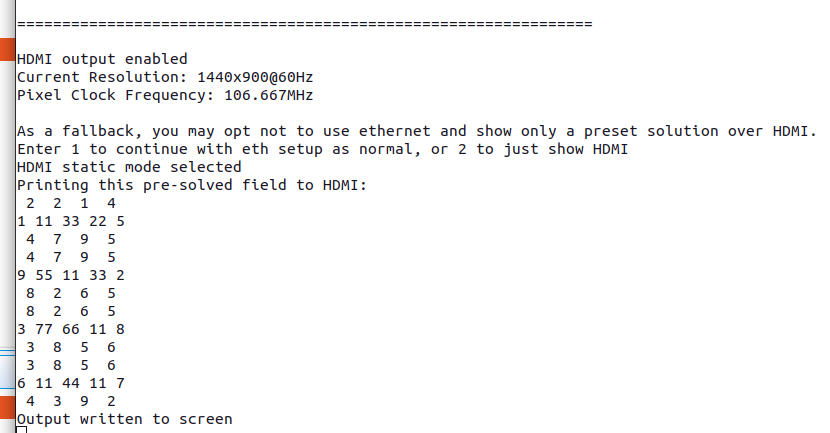
\includegraphics[width=0.5\textwidth]{HDMI_serialout}
  \caption{HDMI output of a preset problem with accompanying serial output}
  \label{fig:hdmi_debug}
\end{figure}

\begin{figure}[h]
  \centering
  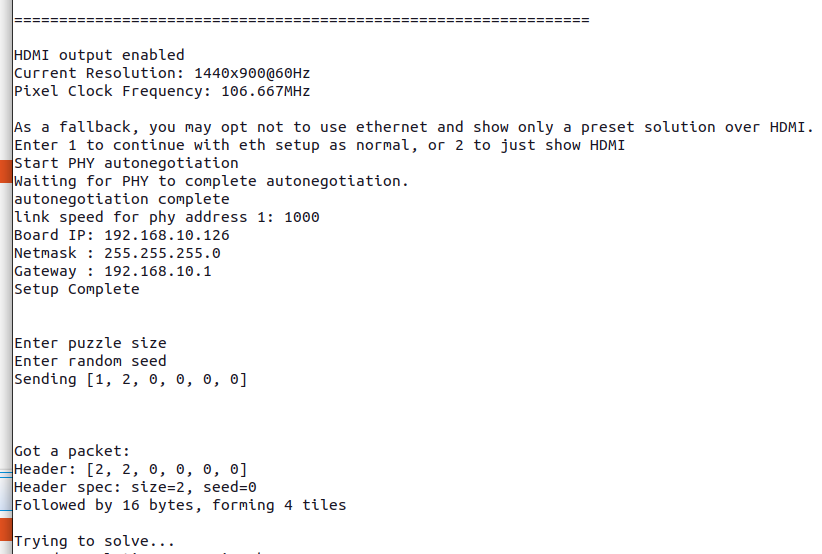
\includegraphics[width=0.5\textwidth]{eth_serialout}
  \caption{Ethernet connection debugging information printed on boot}
  \label{fig:eth_debug}
\end{figure}

On the hardware side, my primary testing process was simply making incremental changes then confirming them by reprogramming the Zybo board and watching its' outputs.
Figure~\ref{fig:hdmi_debug} and figure~\ref{fig:eth_debug} show this.

For benchmarking on hardware, I inserted a timer around the main \verb|solve| call and printed the result to serial.
To benchmark on the host, I used a combination of coreutils' \verb|time| and \href{https://github.com/sharkdp/hyperfine}{hyperfine}.
\href{https://github.com/brendangregg/FlameGraph}{Flamegraph} and \verb|perf| also provided valuable insights into functions which execution was spending the most time in, though these tools were not used to gather the final performance data.

In both cases I tried to run a large array of random inputs in all possible sizes; the means of these runs are shown below.
Supporting this process on my personal machine was a python script to generate puzzle prompts at random, and write them into c headers that I could link into test builds.

\lstinputlisting[language=Python, caption=python prompt generator]{../src/poc/generate.py}

\subsection{Performance}\label{sec:performance}

\begin{figure}[h]
  \centering
  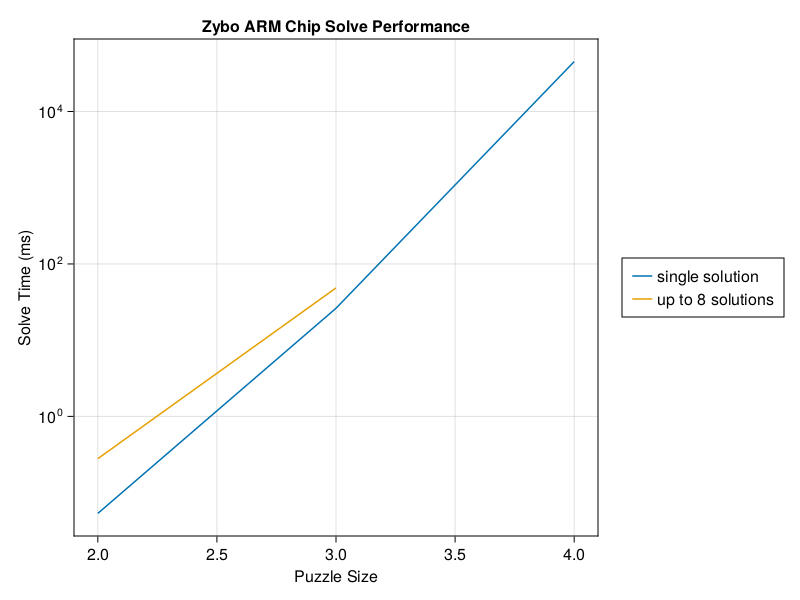
\includegraphics[width=0.8\textwidth]{fpga_perf}
  \caption{Target Hardware Solve Performance}
  \label{fig:fpga_graph}
\end{figure}

\begin{figure}[h]
  \centering
  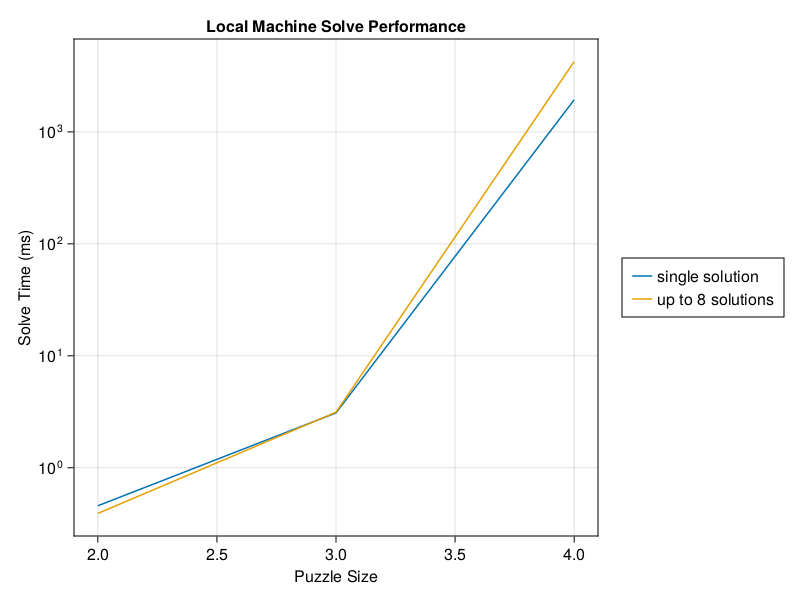
\includegraphics[width=0.8\textwidth]{host_perf}
  \caption{Solve Performance on Personal Device}
  \label{fig:laptop_graph}
\end{figure}

% show graphs from data
% gather data on laptop performance and show
% extrapolate parallel time reduction with parallelism on laptop?

Figure~\ref{fig:fpga_graph} and figure~\ref{fig:laptop_graph} show mean solve time for both single-solution and multi-solution modes on the different hardware.

Several observations can be made:

\begin{enumerate}
  \item Data is only available for puzzle sizes up to 4.
    My solution does not produce predictable output for sizes of 5 and above; on hardware, the solve never terminates.
    I believe this is because the platform does not have enough stack memory available for my method to succeed.
    This obviously heavily limits what relationships we can infer from the data.
  \item Solve time is apparently exponentially related to puzzle size\footnote{``puzzle size'' here is the dimension of \textit{one side} of the game board, that is, a $4 \times 4$ game would have a ``puzzle size'' of $4$ and would contain $16$ tiles.}.
  \item Interestingly, single-solution performance on the target hardware is significantly better than that of multi-solution on the same, but on the laptop this same effect is not reliably present.
    Indeed, multi-solution performance on target hardware was not good enough to reliably record a sample at puzzle size 4.
\end{enumerate}

% what would I have done differently?

\end{document}
